\begin{frame}
\frametitle{Blinn-Phong: Demo}
\begin{figure}[ht]
    \centering
    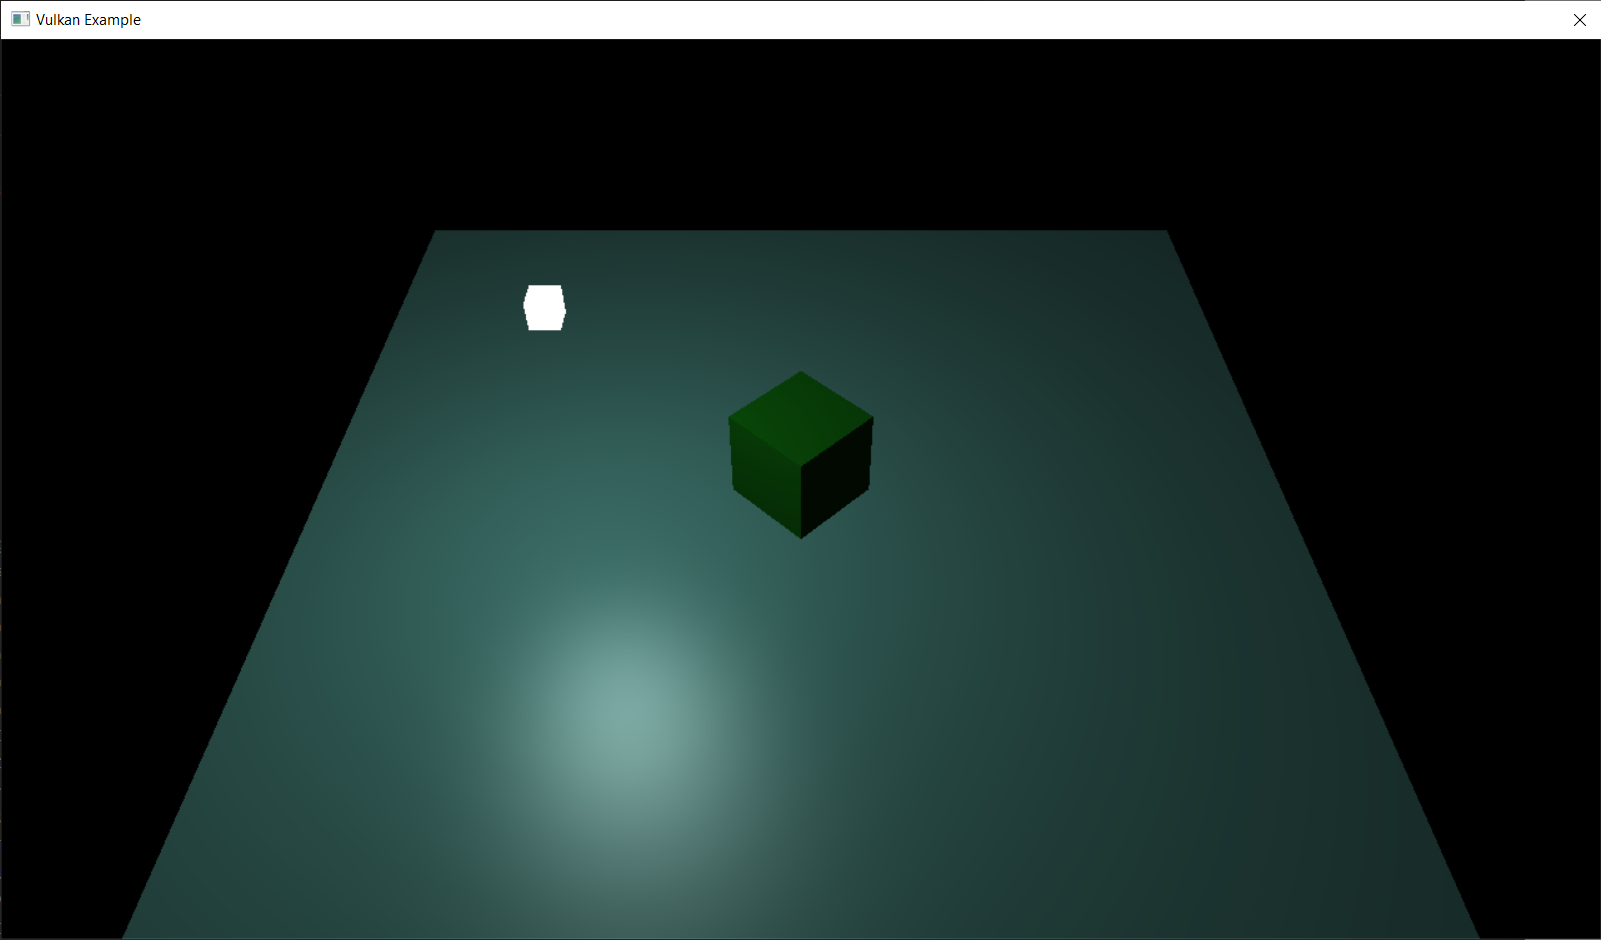
\includegraphics[scale=0.25]{images/SlidesBlinnPhong/SceneMaterialsLight.png}
\end{figure}
\end{frame}

\begin{frame}
\frametitle{Blinn-Phong}
\begin{itemize}
\item L'illuminazione viene divisa in tre componenti: ambient, diffuse e specular
\item La componente ambientale modella il fatto che una scena non è mai totalmente buia
\item La componente diffusiva simula l'impatto che la luce ha sugli oggetti opachi
\item La componente speculare simula il punto luminoso che una luce causa su oggetti lucidi (specular highlight)
\end{itemize}
\end{frame}
